% euphonium_icon.tex -- \euphoniumicon: a small euphonium (bell up, three piston valves, bottom bow, leadpipe with mouthpiece),
%   the mark left of the title (main.tex) and of the README (figs/euphonium_icon.svg, written by gen/mk_icon.sh)
\definecolor{eunavy}{RGB}{31,59,115}
\definecolor{eumid}{RGB}{61,111,180}
\definecolor{eulight}{RGB}{189,215,238}
\tikzset{eutube/.style={draw=eunavy, line width=0.38pt, double=eulight, double distance=#1}}   % a tube: outline and fill
\newcommand{\euphoniumicon}{%
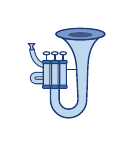
\begin{tikzpicture}[x=1mm, y=1mm, line cap=round, line join=round, baseline={([yshift=-0.6ex]current bounding box.center)}]
  % main tuning slide (left of the valves)
  \draw[eutube=0.44mm] (2.0,5.8) -- (1.0,5.8) arc[start angle=90, end angle=270, radius=0.44] -- (2.0,4.92);
  % leadpipe and mouthpiece
  \draw[eutube=0.44mm] (2.0,6.95) .. controls (1.15,7.15) and (0.65,7.9) .. (0.5,8.95);
  \filldraw[fill=eulight, draw=eunavy, line width=0.38pt] (0.33,8.95) -- (0.67,8.95) -- (0.58,9.42) -- (0.88,9.74) -- (0.02,9.74) -- (0.29,9.42) -- cycle;
  % body: left tube, bottom bow, conical bell stem and bell, one outline
  \filldraw[fill=eulight, draw=eunavy, line width=0.5pt]
    (2.85,4.3) -- (2.85,2.6) arc[start angle=180, end angle=360, radius=2.3]
    -- (7.6,6.8) .. controls (7.7,9.2) and (8.5,10.35) .. (9.75,10.95)
    arc[start angle=0, end angle=-180, x radius=3.1, y radius=0.72]
    .. controls (4.8,10.35) and (5.95,9.2) .. (6.15,6.8) -- (6.35,2.6)
    arc[start angle=360, end angle=180, radius=1.2] -- (3.95,4.3) -- cycle;
  % bell opening
  \filldraw[fill=eumid!70, draw=eunavy, line width=0.5pt] (6.65,10.95) ellipse[x radius=3.1, y radius=0.72];
  \fill[eunavy!85] (6.65,10.86) ellipse[x radius=1.55, y radius=0.33];
  % brace between the valves and the bell stem
  \draw[eunavy, line width=0.42pt] (4.87,6.4) -- (6.2,6.4);
  % three piston valves: casings, caps, stems and finger buttons
  \foreach \x in {2.35, 3.4, 4.45} {
    \filldraw[fill=eulight, draw=eunavy, line width=0.42pt, rounded corners=0.12mm] (\x-0.42,4.35) rectangle (\x+0.42,7.3);
    \filldraw[fill=eumid, draw=eunavy, line width=0.38pt, rounded corners=0.1mm] (\x-0.5,4.05) rectangle (\x+0.5,4.45);
    \filldraw[fill=eumid, draw=eunavy, line width=0.38pt, rounded corners=0.1mm] (\x-0.5,7.2) rectangle (\x+0.5,7.6);
    \draw[eunavy, line width=0.5pt] (\x,7.6) -- (\x,8.35);
    \filldraw[fill=white, draw=eunavy, line width=0.42pt] (\x,8.5) ellipse[x radius=0.43, y radius=0.2];
  }
\end{tikzpicture}}
